\section{Resilient training framework} \label{sec:framework}
Resilient neural networks allow significant performance or 
energy efficiency improvement with little prediction accuracy penalty 
by relaxing the neural network accelerator design constraints. 
This motivates us to obtain more resilient neural networks 
for advantageous accelerator design trade-offs. 
A resilient neural network training framework will be 
detailed in this section. 

\subsection{Overall training framework}
As observed in Section II, we can improve the resilience of 
the neural networks from two aspects. For the problem that the 
computing error patterns are difficult to be captured in training with GPPs, 
we have the accelerators with computing errors integrated into 
the training process. Forward processing influenced by 
the accelerator computing errors is used in training directly 
such that computing error patterns and application data are 
reflected in the neural network models. For the problem that 
some of the layers are affected more than the others, 
we take these layers as critical layers and opt to 
protect the layers from being affected by computing errors. 
With reasonable performance penalty, we can improve the 
overall neural network resilience. 

Following this idea, the overall training framework is depicted in Figure \ref{fig:retrain}. 
Instead of training on GPPs, it has majority of the forward computing performed on the 
accelerators with computing errors while the rest of the training remains on GPPs.
Note that the critical layers should be executed on reliable hardware 
while GPP is one of the options. There are many different approaches 
such as overclocking and lowering voltage that can be used to relax the design constraints.
Although they may cause distinct computing errors, they can be fitted to the 
same training framework.


\begin{figure}
        \center{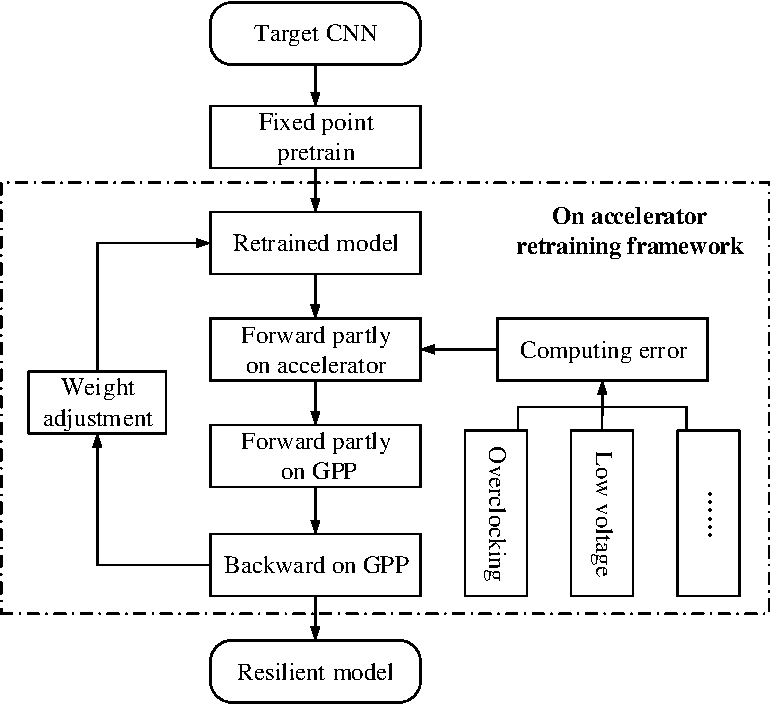
\includegraphics[width=0.85\linewidth]{on_accelerator_retrain_pocess}}
        \caption{Resilient neural network training framework}
        \label{fig:retrain}
%        \vspace{-0.5em}
\end{figure}


\subsection{CNN accelerator abstraction and modification}
As illustrated in the above section, the forward propagation will 
mostly be executed on the CNN accelerator while 
the rest part runs on GPPs. Essentially, the framework targets at a 
heterogeneous computing architecture and frequent 
communication between the accelerator and the GPPs are expected. 
In order to fit various CNN accelerators within the same training framework,
we abstract the CNN accelerators with a high-level interface
which makes the accelerators near transparent to the training framework.
\begin{table*}
        \centering
        \vspace{-0.3em}
        \caption{High-level interface to integrate general CNN accelerators with Caffe}
        \label{tab:api}
        \vspace{-0.3em}
        \begin{tabular}{c|l|l}
                \toprule
                ID & Function Name & Description  \\
                \midrule
                1 & launchAccelerator() & It configures the CNN accelerator and launches it from host CPU. \\
		\midrule
                2 & dataToFPGA(weight, input, wgtDevAddr, inDevAddr) & It transfers both the input data and weight to the FPGA device memory. \\
		\midrule
		3 & dataFromFPGA(outputDevAddr, output) & \shortstack[l]{It transfers all the intermediate output of the CNN layers from FPGA \\device memory to host memory.} \\
		\midrule
		4 & convertIntToFloat(int iData, float fData) & It converts the fixed-point output to float for back propagation processing. \\
		\midrule
		5 & convertFloatToInt(float fData,  int iData) & \shortstack[l]{It converts the floating-point input and weight data to fixed point or \\integer for forward processing on the accelerator.} \\
		\midrule
		6 & dataLayoutReorder(data, reorderedData) & \shortstack[l]{It reorders the data layout for more efficient accelerator execution before \\sending to FPGA device memory.} \\
		\midrule
		7 & dataLayoutRecover(reorderedData, data) & It reorders the output data back to the default format for Caffe back propagation. \\
                \bottomrule
        \end{tabular}
        \vspace{-1em}
\end{table*}



Centering the data communication between the forward propagation 
and the rest of the training framework, we define a high-level 
interface which consists of 7 functions as listed in Table \ref{tab:api}. 
Function 1 is used to launch the CNN accelerator from host. 
Function 2 and 3 are used to transfer data between the host memory and the device memory during 
the training. As the forward propagation on the CNN accelerators is usually fixed point 
and the back propagation on GPPs is floating point, data type converting between fixed point 
and floating point is required. Function 4 and 5 can be used for this purpose. 
Function 1 to 5 are required for all the accelerators. 
Function 6 and 7 are only used for accelerators that compute on reorganized data\cite{pipecnn_2,deepburing_12}. 
With the interface functions, general CNN accelerators can be conveniently 
referenced and used in the proposed on-accelerator training framework. 

In this work, we have the CNN accelerator implemented on Xilinx FPGAs as a case study. 
With Xilinx SDAccel, we can wrap the accelerators with OpenCL API while the accelerators 
can either be developed with OpenCL, HLS or RTL. On top of the OpenCL API, the proposed 
high-level interface can be implemented. Meanwhile, we use Caffe, a C++ based 
deep learning framework, to construct the on-accelerator training framework. With 
both parts developed with C family languages, they can be integrated conveniently. 

%In this work, we have the CNN accelerator implemented on FPGAs.
%Figure 4 depicts the implementation of the training framework on a hybrid 
%CPU-FPGA architecture. In this work, we use Xilinx KCU1500 as the FPGA board 
%and put it on a standard desktop computer. CPU is the controller and it reconfigures 
%the accelerator for a specific CNN structure. In each training iteration, CPU launches 
%the CNN accelerator to perform the forward propagation from bottom layer to top layer. 
%CPU does the backward propagation from top layer to bottom layer. Weights and the image 
%data are initially stored in host memory. It will be transferred to FPGA offchip memory 
%for forward propagation through PCI-E. Similarly, the output data will be transferred 
%from FPGA off-chip memory back to host memory after forward propagation. Because of the 
%OpenCL based API wrapper in SDAccel, the CNN accelerator’s interface can be easily 
%exposed to Caffe for referring to the forward propagation result. 


On top of the high-level interface, the CNN accelerator also needs 
minor modification to enable the on-accelerator training. 
Typically, the training requires the feature map of each neural 
network layer for backward propagation. However, many of the accelerators 
are intensively optimized for inference only and some of the layers’ output 
are fully buffered in on-chip memory to reduce the external memory access. 
In this case, the accelerator should provide an optional data path such that 
intermediate output data can be written to external memory at request.
As shown in Figure \ref{fig:change_of_accelerator}, the output of each layer 
will be transferred to memory using the added optional data path 
when the accelerator is used for training. The write back data path 
can be switched off when the accelerator is used for inference. 

\begin{figure}
        \center{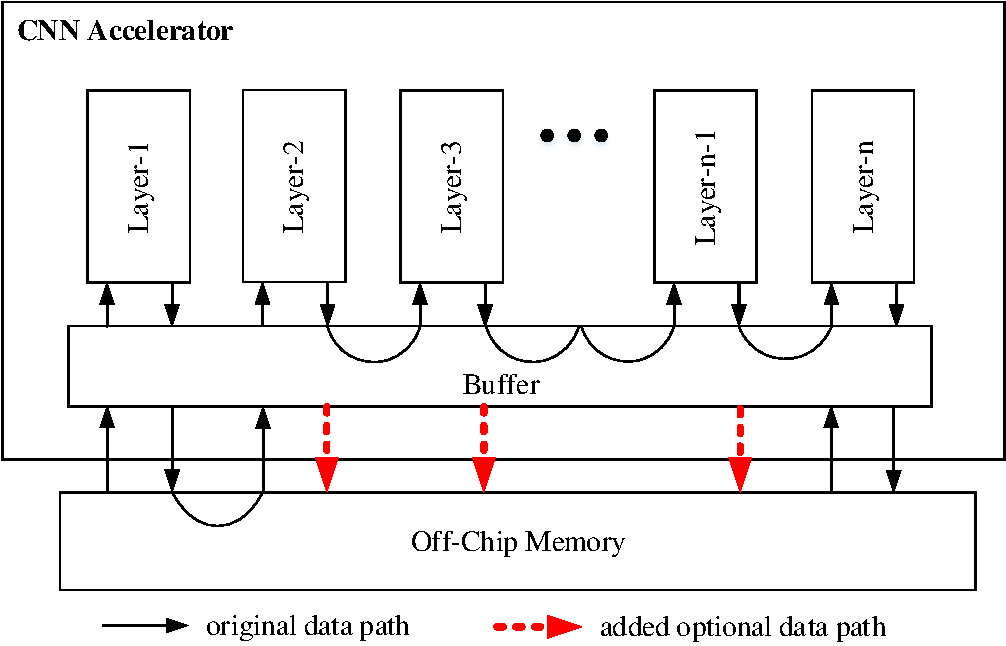
\includegraphics[width=0.85\linewidth]{change_of_accelerator}}
        \caption{Modification of the CNN accelerator data path. It essentially
ensures the feature map of each neural network layer to have an optional data path 
to external memory for back propagation in training.}
        \label{fig:change_of_accelerator}
        \vspace{-1em}
\end{figure}

\subsection{Critical neural network layer protection}
In order to improve the overall neural network resilience, we opt to 
protect the critical network layers and the rest layers can tolerate 
more severe computing errors. The protection is essentially 
to have the critical layers executed on reliable computing infrastructures 
and the exact protection method depends on the target hardware platform.
We may either schedule the critical layers to the GPPs or switch the accelerator 
to reliable mode during the execution of the critical layers.
In this work, we assume GPPs are used for reliable computing 
of critical layers. 

To decide the critical layers of the neural networks, we formulate the 
critical layer section scheme. Suppose the neural network layers include 
$N$ layers and each layer is represented as $L_i$ where $i \in {0, 1, 2, ..., N-1}$.
Then we evaluate the prediction accuracy loss of the neural network 
that have one layer protected on accelerators with computing errors.
When the $i$th layer is protected, the loss is $loss_i$.
Then the most critical layers are the layer that lead to the most 
accuracy loss i.e. $c \in \{k|loss_k = max(loss_i), i \in \{0, 1, ..., N-1\}\}$.

This above formulated approach require large amount of evaluation of 
different layers of the neural network. Instead, we use the actual 
computing errors as the critical layer selection metric. We set an 
error threshold $T$ and assume 8bit integers are used. 
When the error equals to 0, the computing results are correct. 
When the error is larger than $T$, the results are assumed to be large errors.
When the error is wrong but smaller than $T$, the results are considered 
as moderate errors. The layers that include the largest portion of large errors 
are taken as the critical layers.

In addition, scheduling the neural network layers executed 
on the accelerator to GPPs has performance penalty due to the 
computing efficiency gap. As the accelerators are usually 
orders of magnitudes faster than the GPPs for neural network 
processing especially large convolution layers, we can focus on 
the last few small layers to ensure negligible performance 
loss. This constrain greatly reduces the search space
of the critical layers. 


